\chapter{Phylogenetic model of stabilizing selection is more informative about site specific selection than extrapolation from laboratory estimates} 
\label{ch:phylogeny}

\clearpage
\pagebreak

This chapter is an early version of a paper to be submitted to Genome Biology and Evolution and co-authored with Michael A. Gilchrist and Brian C. O'Meara.\\
\newline
\newline
C. Landerer, B.C. O'Meara, M.A. Gilchrist, Phylogenetic model of stabilizing selection is more informative about site specific selection than extrapolation from laboratory estimates

\section{Abstract}
The ever increasing importance of phylogenetics has not been meet with the appropriate developement in models.
Many commonly used phylogenetic models lack biologogical realism.
Models focused on nucleotides are agnostic to selection on higher level selection on codons or amino acids.
Amino acid models on the other hand lack the ability to properly account for mutations.
Codon models try to account for both, mutation and selection, but share that only a single substitution matrix is used, resulting in the same equilibrium frequency at each site.
To remedy this issue, two routes have been taken, the devoplement of more realistic models with site specific selection and the incroporation of supplementary information on site specific selection.
Here we assess and compare the fit and adequacy of phylogenetic inferences made using supplementary information on selection with \selac, a novel codon model of stabilizing selection on amino acids.
We utilize site specific selection parameters for the $\beta$-lactamase TEM estimated via deep mutation scanning to supplement phylogenetic inference to 49 observed sequences.
Using AIC as a measure of model fit, we find that supplementary selection parameters improve model fit compared to classical models without site specific selection ($\DeltaAIC = 289$) but lack model adequacy.
We also highlight that this lack in model adequacy is likely due to biased laboratory conditions.
In contrast, \selac not only provides improved model fit over classical models without site specific selection ($\DeltaAIC = 871$) and experimentally supplemented models ($\DeltaAIC = 582$), it also shows improved model adequacy.
\newpage

\section{Introduction}

Phylogenetic inference is of ever increasing importance across biology \citep{omeara2006,YangAndBourne2009,Ruprecht2017,SchwartzAndSchaffer2017}. 
Most common models used for phylogenetic inference are incorporated into powerful software packages such as RAxML \citep{raxml}, RevBayes \citep{revbayes}, or IQTree \citep{nguyen2015}
While commonly used models are fast and easy to use, they lack biological realism.

Phylogenetic models focused on the nucleotide composition such as GTR, or UNREST \citep{Tavare1986,Yang1994} are limited to mutation effects and are agnostic to any higher level selection on codons or amino acids.
Amino acid models like JTT \citep{jones1992}, BLOSSUM \citep{blossum}, or WAG \citep{whelan2001} attempt to describe the effects of natural selection, however, these do not properly account for mutations between nucleotides and are purely phenomenological.
In an attempt to remedy the shortcomings of nucleotide and amino acid models, codon models combine mutation between nucleotides and selection on the amino acids for which they code.
Most popular are the codon model by \citet{GoldmanAndYang1994} (\gy) and its derivatives.
However, \gy is commonly misinterpreted and provides only a restricted selection scenario that is best described as frequency dependent selection \citep{HughesAndNei1988,Nowak2006,Hughes2007,beaulieu2019}.

One common property of all of these models is the fact that they use a single substitution model across all sites. As a result, every site, whether a nucleotide,  amino acid, or codon, have the same equilibrium distribution.
Biologists, however, have long recognized that equilibrium frequencies and thus the substitution matrix responsible, can vary substantially between sites \citep{felsenstein1981, gojobori1983}.
Individual sites along the sequence often show differences in evolutionary rates, and wide range of preferences for specific amino acids \citep{ashenberg2013, echave2016}.

In response to this variability, \citet{HalpernAndBruno1998} (\hb) provided a general, codon model were each codon site has its own, distinct substitution matrix.
The cost to this generality is the need for 19 amino acid specific selection parameters per site (N.B., the optimal amino acid, by definition, has a selection parameter of 0).
This need for estimating a large number of selection parameters from the sequence data makes the application of \citet{HalpernAndBruno1998} model unfeasible for most studies.
To overcome this parameterization problem,\citet{bloom2014} proposed using data from deep mutation scanning experiments (DMS) as a means of estimating the site specific parameters needed in the \citet{HalpernAndBruno1998}.
Bloom and others \citep{bloom2014, bloom2017, hilton2017} report that using DMS selection parameters greatly improves model fit over models without site specific selection parameters.

The power of DMS stems from the ability to manipulate a large number of individuals in the laboratory and estimate genotype fitness based on frequency changes over many generations.
This, however, limits the application of DMS selection parameters for phylogenetic inference to only organisms which can be cultured in the laboratory and with short generation times.
More troubling is the fact that variation between DMS experiments can lead to significant differences between model fits \citep{hilton2017}.
However, this variation is presumably small compared to the variation between laboratory conditions and those organisms usually encounter in the wild.
As a result, the value of DMS selection parameters for making inferences about sequences evolution in the wild is uncertain.

Instead of using laboratory based selection parameters to mitigate the parameterization issues introduced in \hb, an alternative approach is to simplify the model itself.
For example, Lartillot and colleagues mitigate the high numbers of  parameters required by \hb's codon model using a site categorization approach where a limited, but \emph{a priori} unspecified, number of site categories are estimated from the sequence data \citep{LartillotAndPhilippe2004,le2008,RodrigueEtAl2008,RodrigueAndLartillot2014}.
More recently, \citep{beaulieu2019} introduced a new codon model, \selac, where $20$ site categories are assumed \emph{a priori} to underlie the \hb model.
\selac combines \PC properties and site specific heterogeneity in the strength of selection together using a simplistic nested modeling approach.
Briefly, \selac infers an optimal amino acid for each site and then estimates the selection parameters for the remaining amino acids based on their \PC distance from the optimal amino acid and site specific sensitivity term which is, in turn, treated as a random effect.

We assess and compare the fit and adequacy of phylogenetic inferences made using supplementary DMS selection parameters and \selac. 
We use \phydms \citep{hilton2017} in order to utilize supplementary DMS selection parameters, fitting 49 TEM sequences observed in natural populations of \emph{E.~coli} from \citet{bloom2017}.
Following \citep{bloom2017, hilton2017}, we used the DMS based selection parameters from \citet{stiffler2016} for $\beta$-lactamase TEM to supplement our phylogenetic inference.
TEM is an enzyme found in gram-negative bacteria and catalyzes antibiotics with a $\beta$-lactam ring, providing antibiotic resistance \citep{Neu1969}.
The selection pressure imposed during the DMS experiment was limited to ampicillin and focused solely on the variant TEM-1 \citep{stiffler2016}.
However, TEM variants can also confer resistance to a wide range of other antibiotics \citep{sougakoff1988,sougakoff1989,goussard1991,mabilat1992,chanal1992,brun1994}.

Using AIC as a measure of model fit, as before we find that \phydms outperforms the 228 nucleotide and codon models included in the IQTree package \citep{bloom2014, bloom2017}, but that \selac outperforms \phydms by an additional 582 AIC units.
While very large, our estimate of \DeltaAIC between \selac and \phydms is likely an under estimate given the fact that we, conservatively, counted each inferred amino acid as a separate parameter when calculating \selac's AIC value.
In addition to a superior fit to the observed data, \selac shows higher model adequacy and implies more realistic values of genetic load than \phydms.
We attribute \phydms's poor model adequacy to misappropriation of biased selection parameter estimates from DMS. 
This poor model adequacy, in turn, leads to the unrealistically large estimates of genetic load of the observed TEM sequences.

Together, our results indicate that models can be more informative and applicable than unnatural supplementary data for phylogenetic inference.
\selac, in contrast, provides biological meaningful information such as site specific optimal amino acids and estimates of selection parameters.
In addition, \selac does not rely on supplementary data and is therefore applicable to all alignments of protein coding sequences, and can be expanded to test other hypothesis.


\section{Results}
\subsection{\selac Outperforms Experimentally Informed Models}

We compare \selac and \phydms, two models of site specific stabilizing selection, to 131 nucleotide and 97 codon uniform site models fitted using IQTree \citep[][see Table \ref{tab:AIC_selac} for the best performing models and Table \ref{tab:AIC_full} for all models]{nguyen2015}.
\selac shows the best model fit and provides an improvement of 582 AIC units over the empirically informed model fit by \phydms.
This better performance is in spite of the fact that \selac requires the specification of one optimal amino acid for each of the 263 codons in our TEM alignment.
\phydms, parameterized by site specific selection parameters from \citet{stiffler2016} performs second best and provides an improvement of 289 AIC units for the best uniform site model \emph{SYM}+R2 \citet{zharkikh1994}. 

\selac utilizes a hierarchical model and estimates 263 site specific parameters, $\sim5\%$ of the $19\times N = 4997$ parameters necessary to fully describe site specific selection.
In contrast, \phydms does not infer any site specific parameters from the sequence data, but utilizes site specific selection parameters from DMS experiments.
This is important since $263$ of the $374$ parameters estimated by \selac are the discrete optimal amino acid state at each site. 
As it is unclear if such discrete parameters contribute to the Kullback-Leibler divergence in a similar manner as continuous parameters, it is possible that we are over penalizing.
Therefore, the number of parameters, $n$, for \selac we use is conservative.

\begin{table}
  \centering
  \caption{Model selection, shown are the two models of stabilizing site specific amino acid selection (\selac, \phydms) and the best performing codon and nucleotide model \citep{GoldmanAndYang1994, zharkikh1994}. 
  Reported are the log-likelihood $\log(\Lik)$, the number of parameters estimated $n$, AIC, and $\Delta$AIC values.
  See Table \ref{tab:AIC_full} for results from all models we tested.
}  
  \begin{tabular}{lrrrrrr}
    \hline
    Model							& $\log(\Lik)$ & $n$ & AIC & \DeltaAIC \\ \hline 
    \selac							& -1498 & 374 & 3744 &  0 \\
    \phydms 						& -2061 & 102 & 4326 & 582 \\
    \emph{SYM}+R2 				& -2206 & 102 & 4615 & 871 \\
    \emph{GY94}+F1X4+R2 		& -2243 & 102 & 4690 & 946 \\ \hline
  \end{tabular}
  \label{tab:AIC_selac}
\end{table}

The best performing uniform codon model is \gy \citep{GoldmanAndYang1994}. 
However, \gy is outperformed by 110 nucleotide models like \emph{SYM}+R2.
Like \selac, \gy in its original form, utilizes differences in \PC space between amino acids, but unlike \selac which is a model of stabilizing selection, \gy is best interpreted as frequency dependent selection \citep{HughesAndNei1988,Nowak2006,Hughes2007,beaulieu2019}.

We observe differences in the topology between model fits.
The \selac model is currently too slow to estimate the topology, therefore the topology was estimated using the codon model of \citet{KosiolEtAl07}.
\phydms uses the topology estimated with the codon model of \citet{KosiolEtAl07} as starting point for its topology search.
\phydms diverges from the initial topology suggesting we are conservative in our estimate of $\Delta AIC$ between \selac and \phydms.
However, at this point, it is therefore unclear if  we can attribute the difference in topology solely to the experimentally inferred selection parameters or if other factors contribute.
If we utilize the \phydms inferred topology, with \selac, we find a very similar but slightly worse model fit to our original \selac fit ($\Delta AIC = 2$).
This indicates that the topology has less impact on the model fit than the assumed optimal amino acid sequence, likely due to the short branches and many polytomies in the phylogeny (Figure \ref{fig:phylo_comp}).

Figure \ref{fig:phylo} shows that the estimated phylogenetic trees shift from long terminal branches (\selac) to longer internal branches (\phydms).
While the \selac model fit shows $84 \%$ of all evolution happening at the tips, this reduces $77 \%$ in the \phydms and \gy model fits.
In addition, polytomies are wide spread in all estimated phylogenies, and generally, the shortest branch length are estimated by the symmetric nucleotide model.


\singlespacing
\begin{figure}[H]
     \centering
	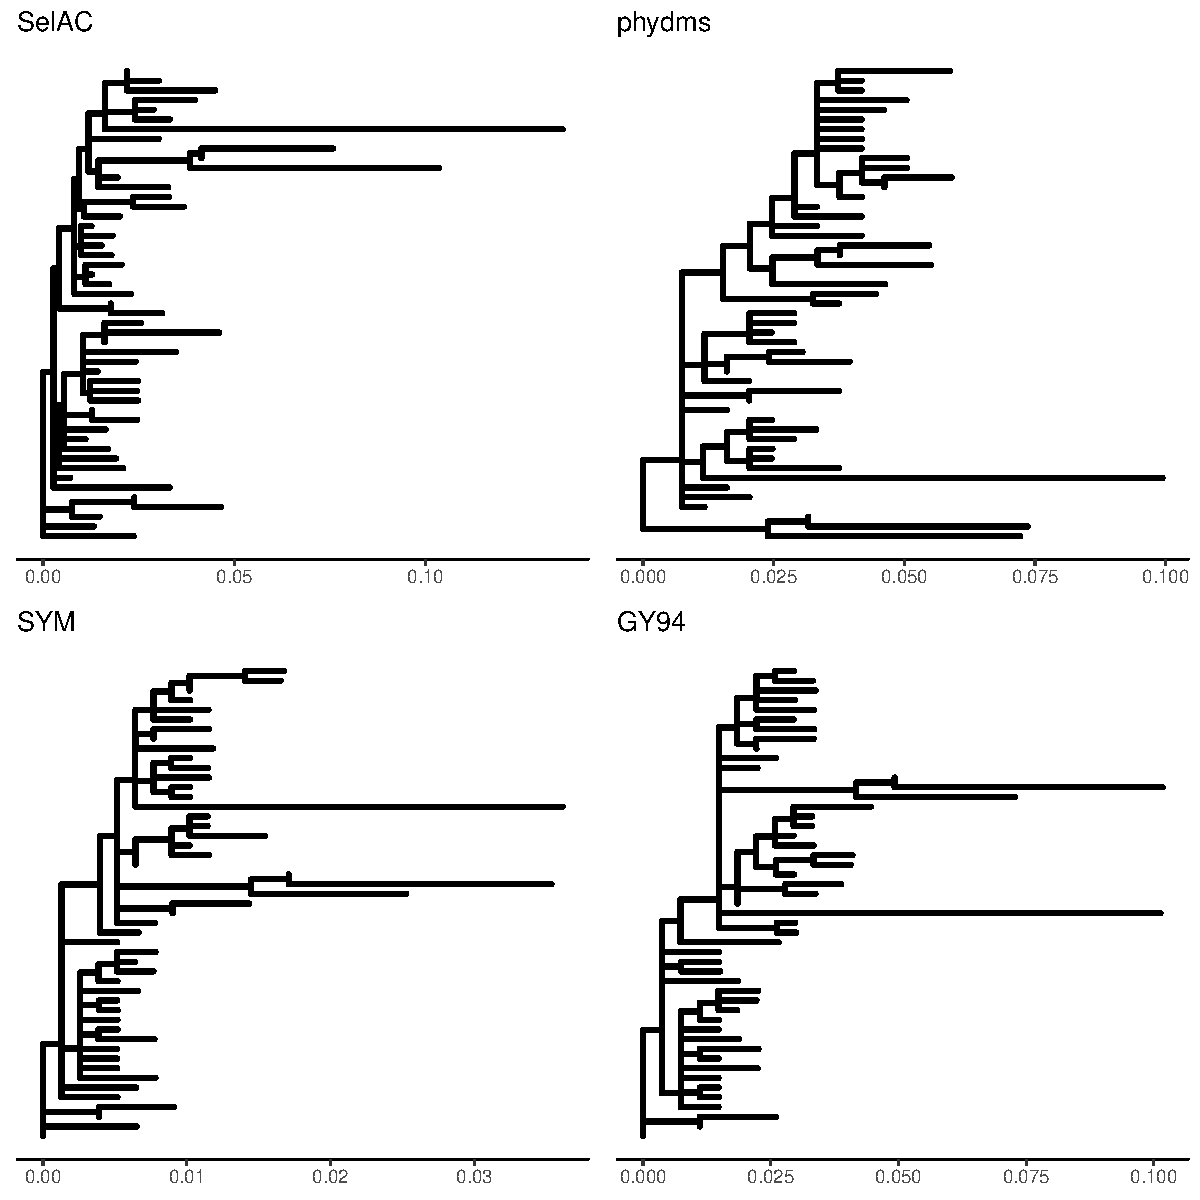
\includegraphics[width=\textwidth]{ch4/phy_TEM2016.pdf}
	\caption{Phylogenies resulting from \selac, phydms, \emph{SYM}, and \gy. As \selac is currently to slow for the inference of topologies, the topology for the \selac phylogeny was inferred using the codon model of \citet{KosiolEtAl07}.}
	\label{fig:phylo}
\end{figure}
\doublespacing
\clearpage


\subsection{Laboratory Inferences Inconsistent with Observed Sequences.}

\singlespacing
\begin{figure}
     \centering
	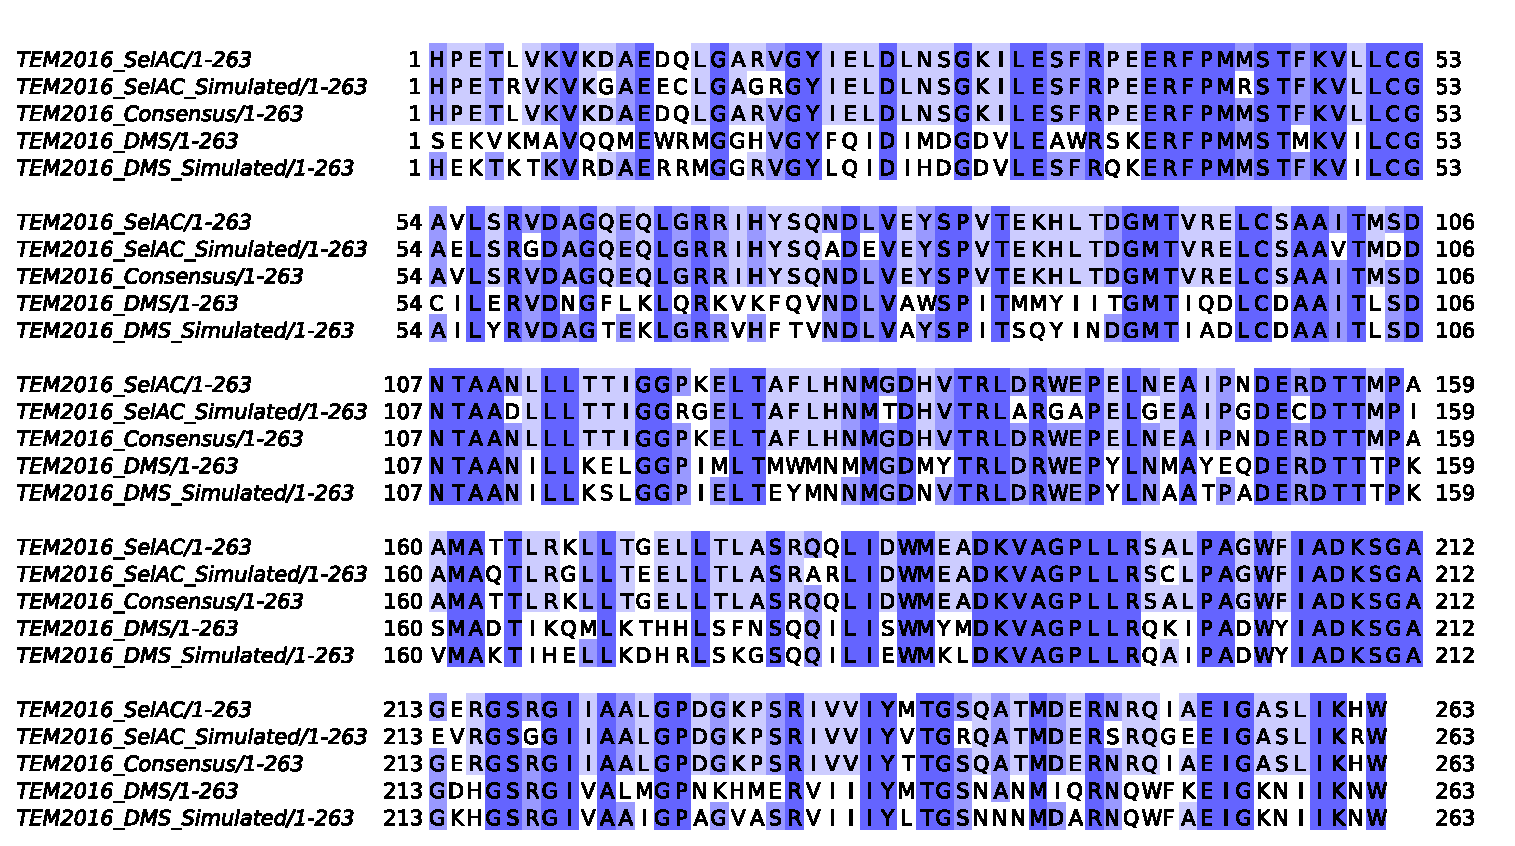
\includegraphics[width=\textwidth]{ch4/seq_simil_all.eps}
	\caption{Alignment of TEM optimal and simulated sequences. Indicated is the percentage identity at each site.}
	\label{fig:sim_seqs_cons}
\end{figure}
\doublespacing

The improved model fits of \phydms relative to more common nucleotide and codon models are, however, deceiving.
The site specific selection inferred by DMS is inconsistent with the observed TEM sequences.
We find that the sequence of selectively favored amino acids has only $52 \%$ sequence similarity with the observed consensus sequence (Figure \ref{fig:sim_seqs_cons}).
In contrast, the sequence of selectively favored amino acids estimated by \selac shows $99 \%$ sequence similarity with the observed consensus sequence.
In addition, assuming the site specific selection estimated by DMS, the observed TEM sequences represent an average sequence specific genetic load of $17.88$ and an average site specific load of $0.065$.

In order to determine if we would expect the observed genetic load under the experimental selection estimates we reconstructed the ancestral TEM sequence and used it as initial conditions for our simulation studies.
We simulate under a wide range of effective population sizes $N_e$, and find that the experimentally inferred site specific selection is very strong.
The estimated ancestral state is identical to the observed consensus sequence.
Simulations of codon sequences under the experimentally inferred site specific selection for amino acids reveal that we would not expect to see the observed TEM sequences.
With an effective population size $N_e$ of $10^7$, we find that the simulated sequences show $62 \%$ sequence similarity to the observed consensus sequence (Figure \ref{fig:dms_sim}a).
Thus, the simulated sequences show a $10 \%$ higher similarity to the observed consensus sequence than the sequence of selectively favored amino acids estimated using deep mutation scanning.

In our simulations, only when $N_e$ is reduced to one individual does drift overwhelm selection (Figure \ref{fig:dms_sim}b).
The genetic load of the simulated sequences decrease slowly with increasing $N_e$.
After simulating until the sequences reached $0.1$ expected mutation per site with an effective population size $N_e = 10^7$ the simulated sequences showed an average sequence specific load of $6.68$ and an average site specific genetic load of $0.025$
This is less than half of the average sequence and site specific genetic load of the observed sequences.
Thus it appears unlikely that the observed sequences have evolved under the DMS inferred site specific selection values.

\begin{figure}
    \centering
    \begin{subfigure}
        \centering
        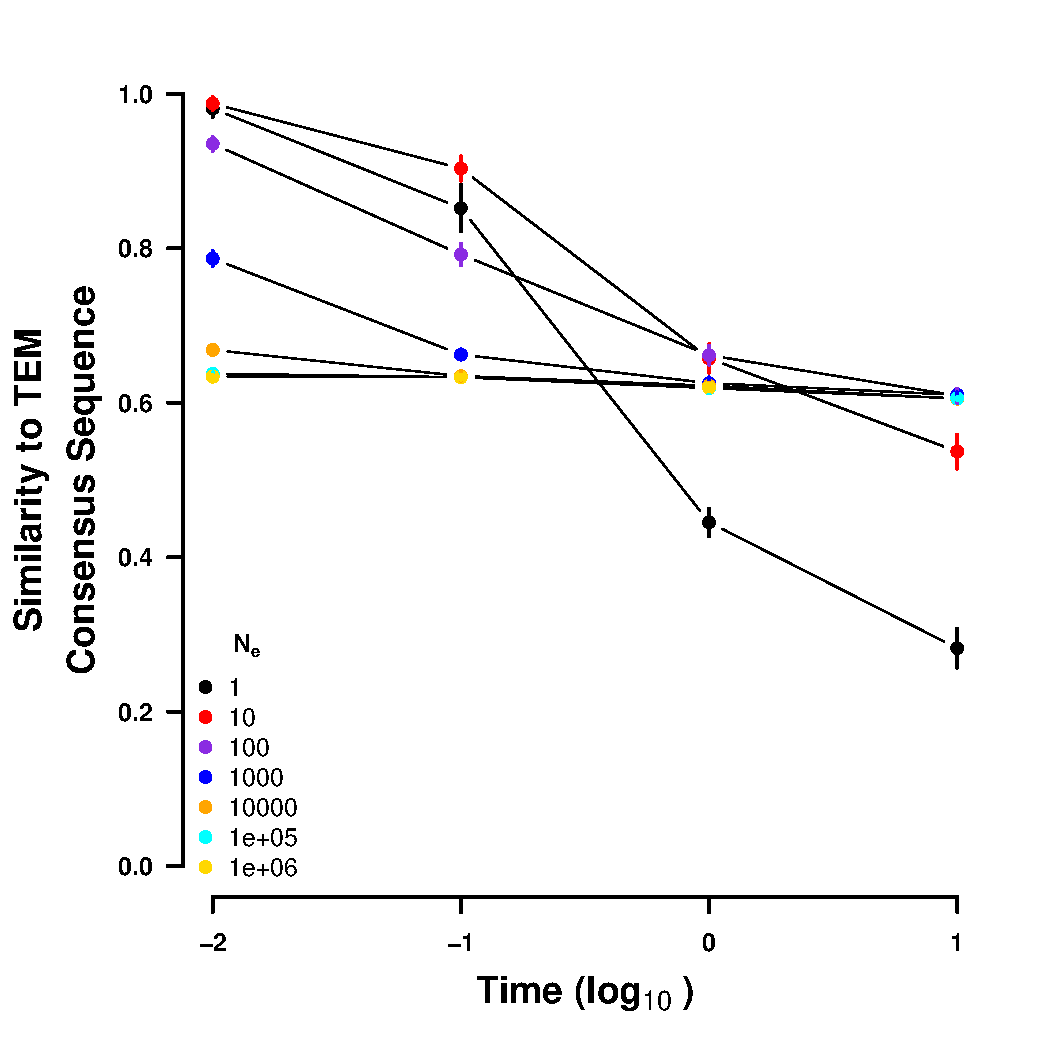
\includegraphics[width=.45\textwidth]{ch4/simulated_dist_time_DMS_ancest.pdf}
    \end{subfigure}
    \begin{subfigure}
        \centering
        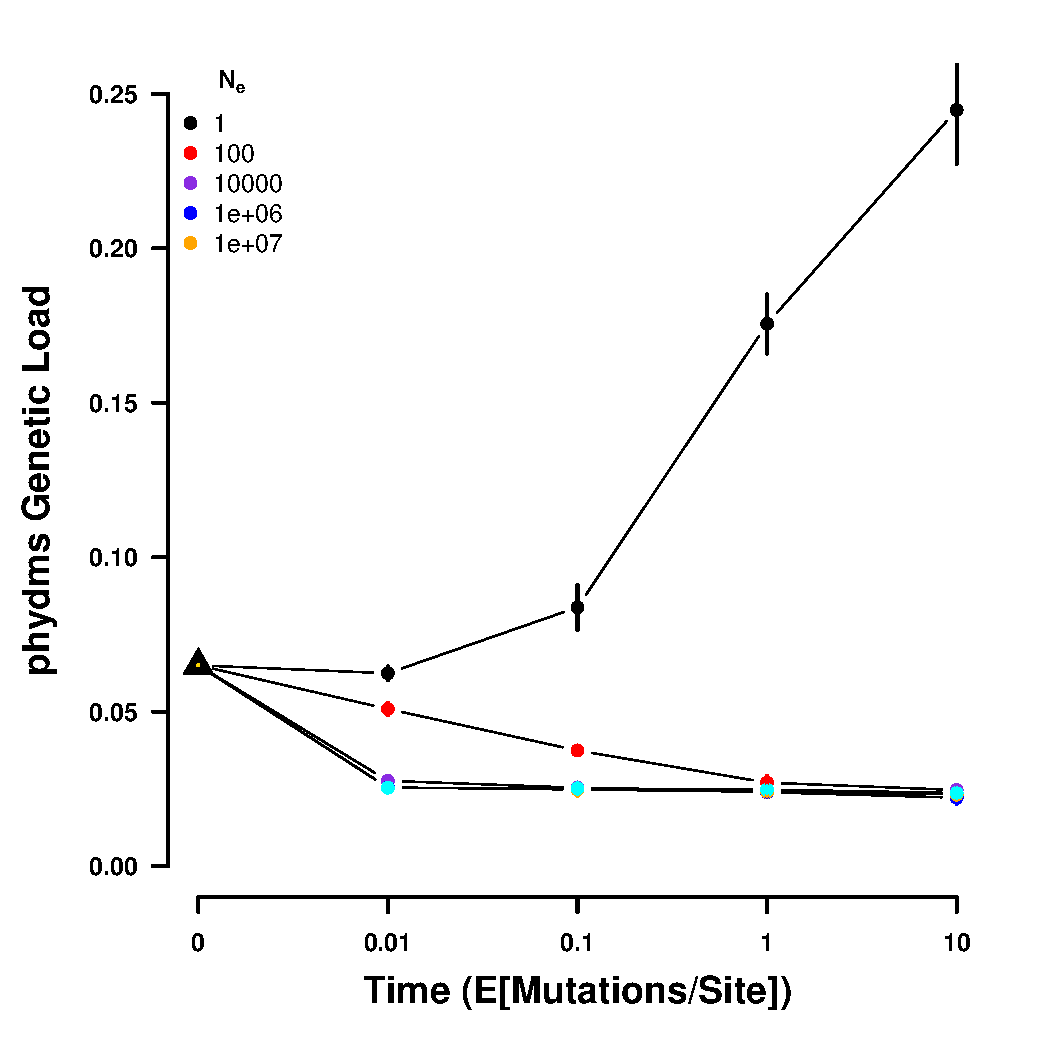
\includegraphics[width=.45\textwidth]{ch4/simulated_gl_time_DMS_ancest.pdf}
    \end{subfigure}
    \caption{Sequences simulated from the ancestral state under the site specific selection on amino acids estimated using deep mutation scanning. 
    (left) Sequence similarity to the observed consensus sequence at various times for a range of values of $N_e$.
    (right) Genetic load of the simulated sequences at various times for a range of values of $N_e$.
    Time is given in number of expected mutations per site, which equals the substitution rate of a neutral mutation.
    Points indicate sample means and vertical bars indicate standard deviations. Initial sequence is the inferred ancestral state of the TEM variants and indicated by a black triangle.}
    \label{fig:dms_sim}
\end{figure}

\subsection{Stabilizing Selection for Optimal Physicochemical Properties Improves Model Adequacy} 
Model adequacy of \selac assessed based on sequence similarity and genetic load and shows that \selac better explains the observed TEM sequences than the experimentally determined site specific selection on amino acids.
The observed consensus sequence has $99 \%$ sequence similarity with the sequence of selectively favored amino acids estimated by \selac, this is in contrast to the average sequence similarity of $98 \%$ among all $49$ observed sequences.
In addition, assuming the site specific selection estimated by \selac, the observed TEM sequences represent an average sequence specific genetic load of $6.4\times10^{-5}$ and an average site specific load of $2.4\times10^{-7}$.

Using the \selac inferred site specific selection and the reconstructed ancestral TEM sequence as initial conditions we simulated codon sequences forward in time for various time periods and $N_e$ values.
As expected, for small $N_e$, simulated sequences drift away from the observed consensus sequence (Figure \ref{fig:selac_sim}a). 
Because of the high similarity between the optimal amino acid sequence estimated by \selac and the observed consensus sequence, the genetic load increases drastically as a result.
Increasing $N_e$ to $10^4$ or above the simulated sequences sequence similarity declines to $83 \%$, indicating that \selac underestimates selection.
After simulating until the sequences reached $0.1$ expected mutation per site with an effective population size $N_e = 10^7$ the simulated sequences showed an average sequence specific load of $1.3\times10^{-5}$ and an average site specific genetic load of $4.8\times10^{-8}$ (Figure \ref{fig:selac_sim}b).
Thus, the simulated sequences show a lower genetic load despite the greater divergence from the observed consensus sequence.
This be an indication that the selection differs between linages.


\begin{figure}
    \centering
    \begin{subfigure}
        \centering
        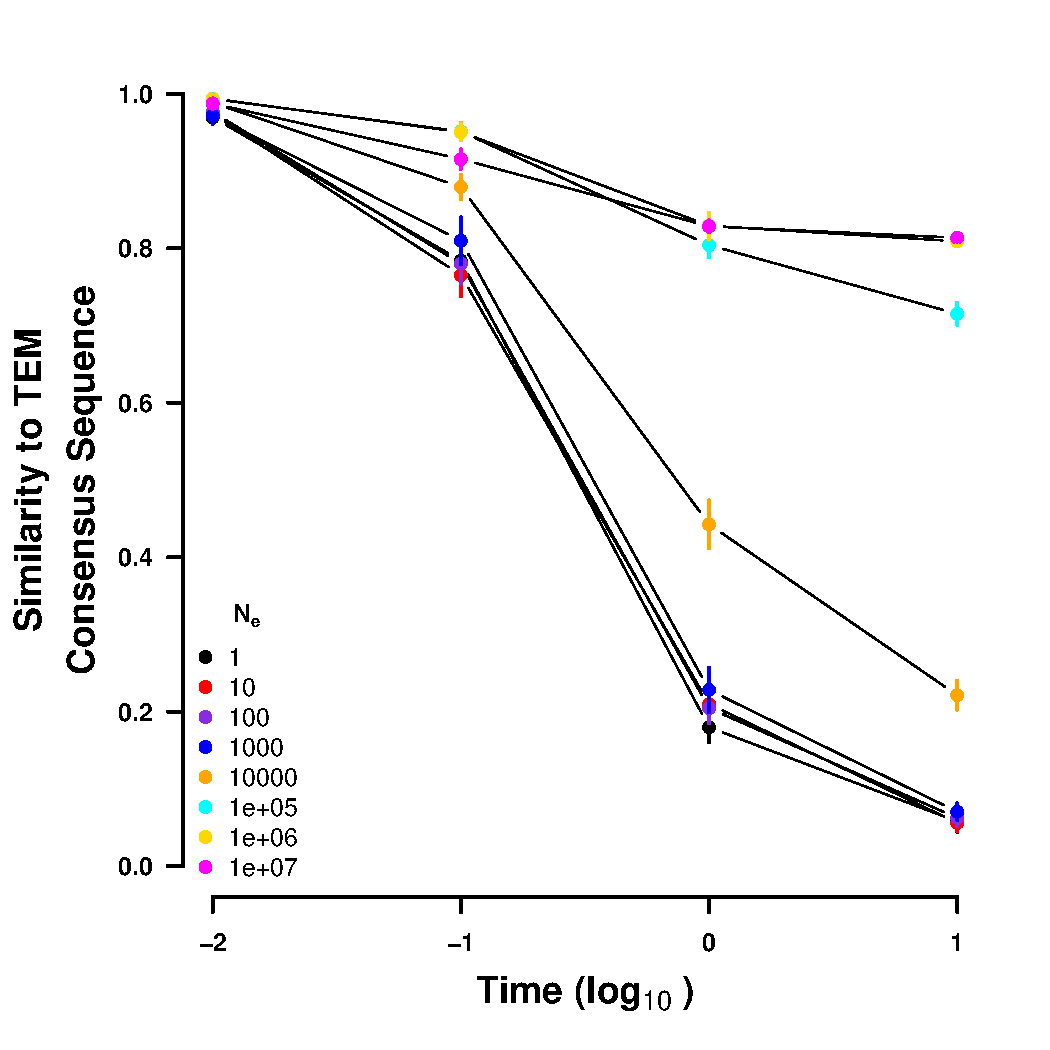
\includegraphics[width=.45\textwidth]{ch4/simulated_dist_time_SELAC_ancest.pdf}
    \end{subfigure}
    \begin{subfigure}
        \centering
        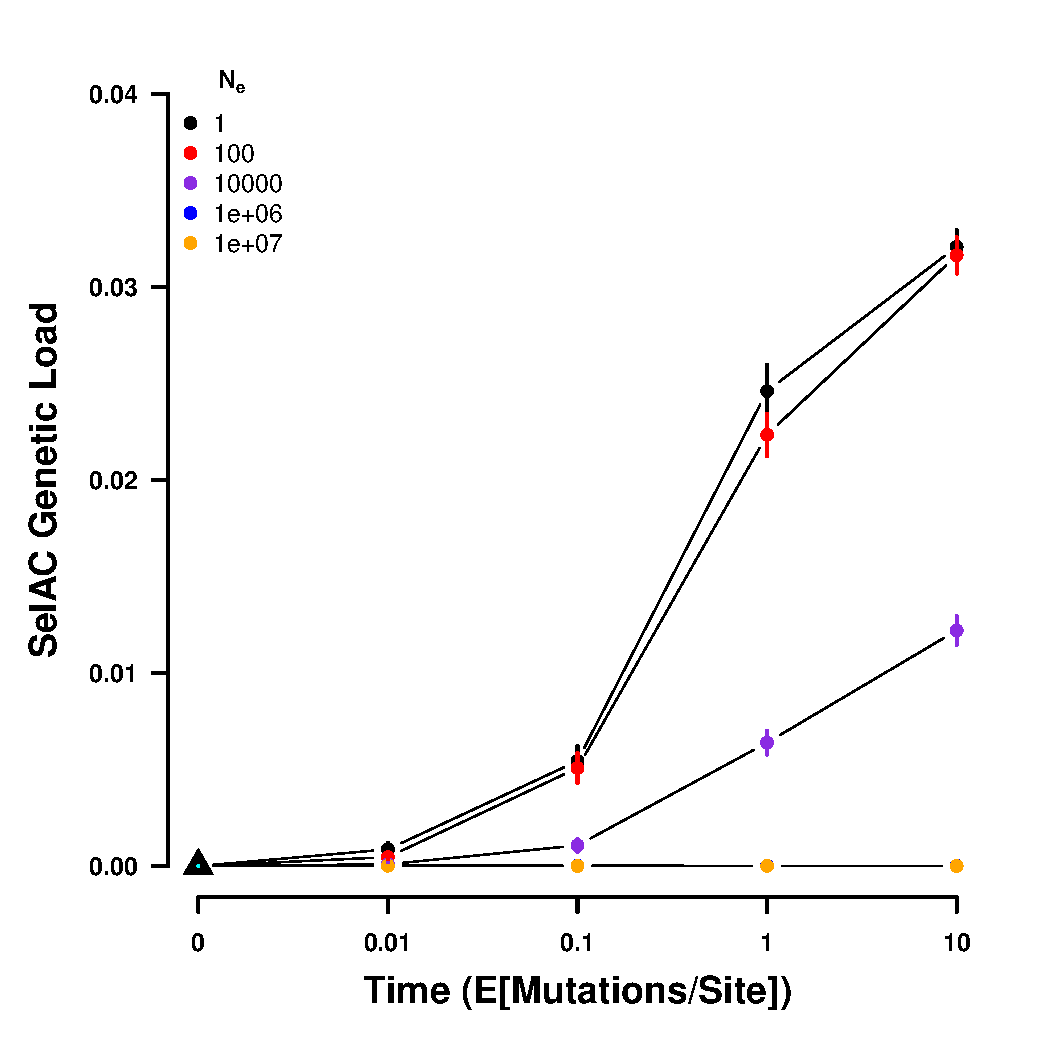
\includegraphics[width=.45\textwidth]{ch4/simulated_gl_time_SELAC_ancest.pdf}
    \end{subfigure}
    \caption{Sequences simulated from the ancestral state under the site specific selection on amino acids estimated using \selac. 
    (left) Sequence similarity to the observed consensus sequence at various times for a range of values of $N_e$.
    (right) Genetic load of the simulated sequences at various times for a range of values of $N_e$.
    Time is given in number of expected mutations per site, which equals the substitution rate of a neutral mutation.
    Points indicate sample means and vertical bars indicate standard deviations. Initial sequence is the inferred ancestral state of the TEM variants and indicated by a black triangle.}
    \label{fig:selac_sim}
\end{figure}

% Random starting point
To further demonstrate the consistency of \selac, we simulated codon sequences over the same time periods using $10$ sequences where codons where sampled uniform.
We find that the sequence similarity increases with effective population size $N_e$.
The random sequences start of with a similarity of $\sim6 \%$ and increase $N_e$ to $\sim28 \%$ (Figure \ref{fig:selac_sim_rand}a).
The same initial sequences simulated under the site specific selection inferred by the deep mutation scanning experiment increase only to $\sim18 \%$ in sequence similarity over the same period of time.


\subsection{Estimating Site Specific Selection on Amino Acids}
\selac allows for the estimation of site specific selection on amino acids and the genetic load of an observed amino acid relative to the inferred optimal amino acid.
Figures \ref{fig:tem2016_sse} and \ref{fig:tem2016_3d} illustrate how the genetic load varies along the TEM sequence.
The region between residue $80$ and $120$, where three consecutive helices are located, consists only of selectively favored amino acids and does not show any genetic load. 
The highest genetic load is found in the unstructured regions and the lowest genetic load is found in $\beta$-sheets.
However, this difference is not statistically significant ($p = 0.17$).
The largest increase in genetic load is located at the beginning of the last helix.
This region strongly contributes to the estimate of similar genetic loads for helices and unstructured regions in the observed TEM sequences (Table \ref{tab:selection}).
However, exclusion of this site as outlier does not yield significance ($p = 0.09$).

\selac assume that the efficacy of selection $G$ is $\Gamma$-distributed with a mean of $1$. 
However, it is possible to estimate site specific values using the parameters estimated by \selac.
We constraint $G$ to a maximum value of $300$ in all cases.
While this biases our estimate of $G$, the bias is consistent across all estimates and does not prohibit the comparison of $G$ terms.

The highest efficacy of selection $G$ is estimated in the $\beta$-sheet regions which is consistent with the lowest genetic load in these regions.
Residues forming the substrate binding site appear to be under the strongest selection, with no accumulated genetic load.
However, this is not the case for the two active sites.
We find in one sequence (\textit{Acinetobacter baumannii}, TEM-193) a Lysine, a proton donor, at the proton acceptor site 143 driving the reduced efficacy of selection $G$. 
This is in concordance with the experimental DMS estimates, where proton acceptors are selectively favored.
Again, any differences between secondary structure elements are not statistically significant.

\begin{table}
  \centering
  \caption{Efficacy of selection ($G$) and genetic load for TEM and SHV, and separated by secondary structure. $G$ was estimated as a truncated variable with an upper bound of 300.}
  \begin{tabular}{llrrrrr}
    \hline
    & & & \multicolumn{2}{c}{$G$} & \multicolumn{2}{c}{Genetic Load $L_i$} \\ 
    Protein & Secondary Structure & \# Residues	& \multicolumn{1}{c}{Mean} & \multicolumn{1}{c}{SE} & \multicolumn{1}{c}{Mean} & \multicolumn{1}{c}{SE} \\ \hline 
    TEM	&		& 263 & 219.3 & 7.5  & $15.9\times10^{-8}$ & $6.5\times10^{-8}$ \\
    &Helix 		& 113 & 206.1 & 12.4 & $17.5\times10^{-8}$ & $13.1\times10^{-8}$ \\
    &$\beta$-Sheet 	&  48 & 238.6 & 15.8 & $ 6.8\times10^{-8}$ & $2.9\times10^{-8}$ \\
    &Unstructured 	& 102 & 224.8 & 11.4 & $18.6\times10^{-8}$ & $8.1\times10^{-8}$ \\
    &Active/Binding Sites 	&   5 & 202.6 & 62.2 & $0.01\times10^{-8}$& $0.01\times10^{-8}$ \\ \hline
    
    SHV&		& 263 & 244.9 & 6.8  & $4.0\times10^{-8}$ & $1.9\times10^{-8}$ \\
    &Helix		& 102 & 234.6 & 11.5 & $7.3\times10^{-8}$ & $4.8\times10^{-8}$ \\
    &$\beta$-Sheet 	&  66 & 253.1 & 12.8 & $2.1\times10^{-8}$ & $1.1\times10^{-8}$ \\
    &Unstructured	&  95 & 224.7 & 11.4 & $1.5\times10^{-8}$ & $0.6\times10^{-8}$  \\
    &Active/Binding Sites	&   5 & 239.9 & 60.0 & $1.5\times10^{-8}$ & $1.5\times10^{-8}$ \\ \hline
  \end{tabular}
  \label{tab:selection}
\end{table}


\singlespacing
\begin{figure}
     \centering
	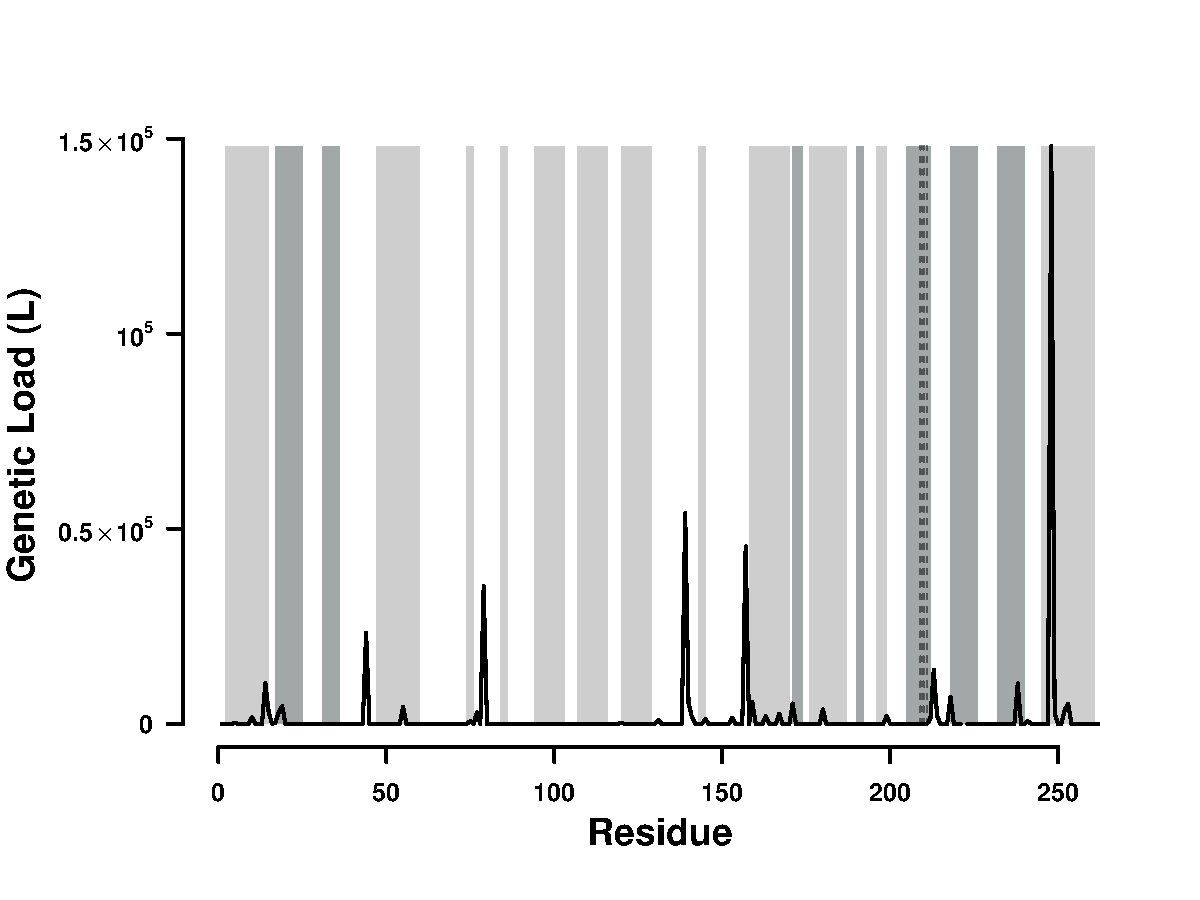
\includegraphics[width=\textwidth]{ch4/GL_slide_TEM2016}
	\caption{Distribution of average site specific genetic load in TEM over all observed TEM variants. 
	Average site specific genetic load is indicated by the black line. 
	Light gray bars indicate where helices are found, and dark gray bars indicate $\beta$-sheets.
	The three residues forming the binding site and the two residues forming the active are indicated by triangles at the top of the plot.}
	\label{fig:tem2016_sse}
\end{figure}
\doublespacing

It was previously proposed that experimentally inferred site specific selection for amino acids can be used to extrapolate the fitness landscape of related proteins \citep{bloom2014, bloom2017}.
We therefore compared the genetic load, the \selac selection parameters of our \selac TEM model fit to a \selac model fit of SHV, and site specific efficacy of selection $G$.
The genetic load observed in SHV sequences appears to be lower than in TEM with the exception of residues found in $\beta$-sheets and the active site (Table \ref{tab:selection}).
This is consistent with the elevated efficacy of selection $G$ in SHV.
However, only differences in genetic load in the unstructured regions are significantly different between the TEM and SHV sequences, but only at the $\alpha = 0.05$ significant level ($p = 0.04$).
While the average genetic load across secondary structures is not significantly different, the sites causing increases genetic load differ between SHV and TEM (Figure \ref{fig:shv2016_sse}).
In contrast to TEM, we find the highest genetic load among SHV secondary structure features in the helices (Table \ref{tab:selection}).
The highest genetic load in SHV is observed at the end of the first helix.
We do find a peak of similar magnitude in the TEM sequence at the end of the first helix, but this peak is overshadowed by the increased genetic load at the beginning of the last helix.

We find that the site specific efficacy of selection $G$ differs greatly between SHV and TEM ($\rho = 0.12$), despite a similar estimate of $\alpha_G$ describing the distribution of $G$ values (Figure \ref{fig:tem_shv_param_comp}a).
Most \selac selection parameters are very similar between the TEM and the SHV model fit. 
An exception is the weight for the \PC composition property $\alpha_c$ (Figure \ref{fig:tem_shv_param_comp}b).
Furthermore, we find that the sequences of selectively favored amino acids estimated by \selac for TEM and SHV only show $68 \%$ sequence similarity.
These results indicate that the extrapolation from one proteins fitness landscape to another is problematic. 


\section{Discussion}

Here we revisited how well site specific estimates of selection from deep mutation scanning experiments inform sequence evolution and compared it to \selac, a novel phylogenetic model of stabilizing selection.
Previous work has shown that laboratory estimates of selection can improve model fit over classical approaches like GY94 \citep{bloom2014, bloom2017}.
While our study confirms this notion, we identify important shortcomings of these laboratory estimates for phylogenetic studies.
In contrast, \selac is a phylogenetic model of stabilizing selection based on \PC properties and does not require costly laboratory estimates of selection and is, nevertheless, favored by model selection (Table \ref{tab:AIC_selac}).
More specifically, it estimates site specific selection on amino acids from the sequence data based on distances between amino acids in \PC space \citep{grantham1974,beaulieu2019}.
This allows \selac to be applied to any set of protein coding sequences, eliminating the need to extrapolate from one homologous gene family to the next (e.g. from TEM to SHV).
In addition this generality allows for the comparison of model parameters for these proteins.

While previous work showed the advantages of experimentally informed phylogenetics, they did not assess how adequate the estimated selection reflects observed wild-type sequences.
The low sequence similarity between the observed consensus sequence and the sequence of selectively favored amino acids estimated by deep mutation scanning experiments is evidence for that.
This begs the question how well the experimental selection coefficients represent selection on these sequences in nature.
Deep mutation scanning experiments are performed using a comprehensive library of mutants and a strong artificial selection pressure \citep{FirnbergAndOstermeier2012, Jain2014, FowlerAndFields2014, Fowler2014}.
This results in  very large selection coefficients $s$ and a heterogeneous population of competing individuals unlikely to occur in nature.

The selection pressure imposed during the DMS experiment was limited to ampicillin and focused solely on TEM-1 \citep{stiffler2016}.
However, TEM variants can also confer resistance to a wide range of other antibiotics, including penicillins, cephalosporins, cefotaxime, ceftazidime, or aztreonam \citep{sougakoff1988,sougakoff1989,goussard1991,mabilat1992,chanal1992,brun1994}.
Thus, the inferred selection is biased towards ampicillin and is inconsistent with the observed TEM sequences (Figure \ref{fig:dms_sim}).
This may very well be appropriate to explore the selection on TEM in a hospital environment but is unlikely to be representative of the selection faced by \ecoli and other gram-negative bacteria in nature.
%We therefore propose to include a variety of selection pressures if the experimental selection estimates are used for phylogenetic inference.

%TODO:  Lack of repeatability between labs introduces further problems (Firnberg et al 2014 vs. Stifler et al. 2016).

If we assume that the DMS selection coefficients underly the evolution of the observed TEM sequences we can think of two possible explanations for the observed sequences.
First, the sequences are unable to reach a fitness peak, potentially due to a weak selection pressure or not enough time.
Alternatively, the TEM sequences found in nature are highly maladapted, yet with very similar sequences.
Both explanations seem unlikely.
For example, \ecoli has a large effective population size $N_e$, estimates are on the order of $10^8$ to $10^9$ \citep{OchmanAndWilson1987, hartl1994}.
%As new mutations are introduced into a population at a rate proportional to $N_e$, \ecoli can effectively explore the sequence space.
We, therefore, expect the observed sequence variants to be near mutation-selection-drift equilibrium.
This expectation is supported by our simulations in which we observe a higher sequence similarity with the observed TEM consensus sequence and decreased genetic load even with much smaller $N_e$ (Figure \ref{fig:dms_sim}).
Furthermore, previous work showed that the catalytic reaction performed by TEM of penicillin-class antibiotics is close the diffusion limit.
As a result some researchers refer to TEM as a perfect enzyme \citep{matagne1998,stiffler2016}.
The very large effective population size, however, also raises a concern that the population mutation rate of \ecoli $\Theta = 4N_e\mu$ exceeds $0.1$ and, thus, violated \selac's weak mutation assumption \citep{deKoning259507}.
If the weak mutation assumption is violated evolution is no longer mutation limited and the time between fixation events increases.
However, \phydms operates under the same weak mutation assumption and the experimentally inferred selection clearly violates the weak mutation assumption.

As experimental selection estimates are not readily available for most organisms and proteins, a possible approach is the extrapolation of empirical estimates to homologous gene families \citep{bloom2014, bloom2017}.
When extrapolating the selection estimates from the $\beta$-lactamase family TEM to the SHV family, the sequence similarity between the observed consensus sequence and the sequence of selectively favored amino acids estimated from deep mutation scanning experiments drops only slightly from $52 \% $ to $49 \%$.
This may have contributed to the notion that extrapolation to homologous gene families is possible.
In contrast, estimates of site specific efficacy of selection $G$ revealed large differences in the site specific selection on amino acids between TEM and SHV.
The mismatched \PC weights further indicate differences in selection constraints. 
While the polarity of amino acids is of similar importance in TEM and SHV, amino acid composition appears to play a much greater role in SHV than in TEM.
In contrast to the experimental selection estimates, extrapolated from TEM to SHV, the \selac selection estimates are consistent with the observed sequences, e.g. the selectively favored amino acids estimated by \selac shows a high sequence similarity with the observed TEM and SHV consensus sequence ($99 \%$).
Furthermore, \selac allows to compare parameters between fits to homologous proteins instead of relying on extrapolation.

While \selac better explains the observed TEM sequences than the experimental estimates of site specific selection on amino acids, it is not without shortcomings itself.
\selac is currently to slow to be used in topology searches, therefore it is unclear if the differences in topology between \phydms and \selac can be attributed to the same inadequacies of experimentally inferred selection.
The formulation and implementation of \selac can and should be improved upon as the simulation of TEM evolution from the ancestral state under the \selac inferred site specific selection revealed.
Starting from the ancestral sequence, the simulated sequences diverge despite stabilizing selection for the optimal amino acid, indicating that \selac may underestimate selection.
While \selac allows for site heterogeneity in selection for amino acids, it still ignores epistasis.
This however, is a shortcoming that is shared with experimental estimates as each mutant typically only carries one mutation \citep{FirnbergAndOstermeier2012, Jain2014}.
Furthermore, not every protein is under stabilizing selection, however, \selac is a model stabilizing selection and may therefore not be adequate for every protein.
TEM plays a role in chemical warfare with conspecifics and other microbes, therefore some sites may be under negative frequency dependent selection.
This potential heterogeneity in selection highlights another shortcoming of \selac.
\selac assumes the same distribution for the efficacy of selection $G$ and \PC sensitivities across the whole protein.
However, it possible that residues in different secondary structures or at active sites do not share a common distribution.

% TODO: talk about that random sequences still have 30% functionallity under selac. Could explain why the  simulation from the ancestral state diverges to ~80 %. Or maybe do we underestimate selection?

As \selac assumes that the fitness of an amino acid at a site declines with its distance in \PC space to the optimal amino acid, the choice of \PC properties becomes important.
In this study, we used composition, polarity, and molecular volume \citep{grantham1974} for all sites and only estimated their weighting.
However, a wide range of additional \PC properties of amino acids have been described \citep{Kawashima2008}.
A more optimal choice of \PC properties may be possible as well as relaxing the assumption that the same properties apply to all sites equally.
%Future work will attempt to address these shortcomings, however, \selac's hierarchical model structure and the open-source code base allow researchers to easily address these and other shortcoming how they see fit.

In conclusion, experimental estimates of site specific selection on amino acids have to be treated with skepticism and their adequacy should be assessed before using them to inform phylogenetic inferences.
This study was initiated to assess the quality of \selac with the expectation that \selac could be a faster, cheaper, and more readily available alternative to experimentally inferred selection;
specifically in organisms where these experiments are not feasible.
Intuitively one would expect that selection coefficients of mutations estimated in living organisms would provide more information on the evolution of proteins than a model relying on many simplifying assumptions.
As we show in this study, not only can \selac estimate site specific selection on amino acids but our approach is a more adequate description of selection on amino acids in nature than experimental estimates.


\section{Materials and Methods}

\subsection{Phylogenetic Inference and Model selection}

TEM sequences were obtained from \citet{bloom2017} already aligned.
Experimentally selection parameters for TEM were taken from \citet{stiffler2016}.
We followed \citep{bloom2017} to convert the experimental selection parameters into site specific equilibrium frequencies for \phydms. 
\phydms (version 2.5.1) was fitted to the site specific selection from \citet{stiffler2016} using python (version 3.6).
\selac (version 1.6.1) was fitted to the TEM alignment using R (version 3.4.1) \citep{rcore}.
We assumed the \PC properties estimated by \citet{grantham1974} and only estimated the weighting terms for each property from the data.
We choose the constraint free general unrestricted model \citep{Yang1994} as mutation model for \selac.
All other models were fitted using IQTree \citep{nguyen2015}.
We report each model's $\log(\Lik)$, and AIC.
Models were selected based on the AIC values.

\subsection{Sequence Simulation}

Sequences were simulated by stochastic simulations using a Gillespie algorithm \citep{gillespie1976} that was model independent.
To calculate fixation probabilities during the simulation we followed \citet{SellaAndHirsh2005}.
The selection parameters were estimated using \selac or taken from \citet{stiffler2016}.
We choose the selection parameters resulting from the highest concentration (2500 $\mu g/mL$) treatment of ampicillin for our comparison.
We rescaled the experimental selection parameters such that the amino acid with the highest fitness at each site has a value of one.
Mutation rates for the simulations were taken from the \selac.
The initial sequences was the ancestral sequence reconstructed using FastML \citep{fastml} (last accessed: 30.09.2018).
Each sequence was simulated 10 times and we report average genetic load and sequence similarity and the standard error.
The sequences were sampled at times 0.01, 0.1, 1, and 10 expected mutations per site.

\subsection{Estimating site specific selection parameters $w_i$}

Following \citet{beaulieu2019} $w_i$ is proportional to
\begin{equation}
w_i \propto \exp(-A_0\eta\psi)
\end{equation}
where $A_0$ describes the decline in fitness with each high energy phosphate bond wasted per unit time, and $\psi$ is the protein's production rate.
$\eta$ is the cost/benefit ratio of a protein (see \citep{beaulieu2019} for details). 
However, \selac only estimates a composition parameter $\psi' = A_0\psi N_e$ thus
\begin{equation}
\psi = \frac{\psi'}{A_0N_eq}
\end{equation}
\selac assumes that the effective population size $N_e = 5\times 10^6$ and that $A_0 = 4 \times 10{-7}$ \citep{gilchrist2007}.

\subsection{Model Adequacy}

Model adequacy was assessed by comparing the observed sequences and simulations under the site specific selection inferred by the deep mutation scanning experiment or \selac.
First, similarity between the sequence of selectively favored amino acids and the observed TEM sequences was assessed.
Sequence similarity was measured as the number of differences in the aligned amino acid sequences.
Second, the genetic load of the observed and the simulated sequences was calculated using either the site specific selection inferred by the deep mutation scanning experiment or \selac.
The average genetic load for site $i$ in the alignment was calculated as
\begin{equation}
L_i = \frac{w_{max,i} - \overline{w_i}}{w_{max,i}}
\end{equation}
where $w_{max,i}$ is the fitness of the selectively favored amino acids at position $i$, either estimated using the site specific selection inferred by DMS or \selac.
We, however, rescaled all fitness estimates such that $w_{max,i} = 1$
$\overline{w_i}$ represents the average fitness of the residues observed at position $i$.
The average sequence specific genetic load $L$ was calculated as the sum of the site specific genetic loads $L = \frac{1}{n}\sum_{i=1}^n L_i$ where $n$ is the number of amino acid sites.

\section{Acknowledgments}

This work was supported in part by NSF Award and DEB-1355033 (BCO, MAG, and RZ) with additional support from The University of Tennessee Knoxville. 
CL received support as a Graduate Student Fellow at the National Institute for Mathematical and Biological Synthesis, an Institute sponsored by the National Science Foundation through NSF Award DBI-1300426, with additional support from UTK. 
The authors would like to thank Russel Zaretzki, Jeremy Beaulieu and Alexander Cope for their helpful criticisms and suggestions for this work.



\clearpage
%\beginsupplement
\section{Appendix: Supplementary Material}

\singlespacing
\begin{longtable}{clrrrrrr}
  \caption{Model selection of 229 models of nucleotide and codon evolution.}
  \label{tab:AIC_full}
  \\ 
  \toprule
  No. & Model & $\log(\Lik)$ & n & AIC & \DeltaAIC  \\   \hline \endfirsthead
  \caption*{Table \ref{tab:AIC_full} Continued}\\\toprule
  No. & Model & $\log(\Lik)$ & n & AIC & \DeltaAIC  \\   \hline \endhead
  \hline \endfoot
  \bottomrule
  \endlastfoot

	1 & \selac+G4 & -1497.971 & 374 & 3743.942 & 0 \\ 
	2 & \phydms & -2060.85 & 102 & 4325.7 & 582 \\ 
	3 & SYM+R2 & -2205.877 & 102 & 4615.754 & 871.754 \\ 
	4 & TIMe+R2 & -2232.406 & 100 & 4664.811 & 920.811 \\ 
	5 & TVMe+R2 & -2232.838 & 101 & 4667.677 & 923.677 \\ 
	6 & TIM3e+R2 & -2234.332 & 100 & 4668.664 & 924.664 \\ 
	7 & TIM2e+R2 & -2234.381 & 100 & 4668.763 & 924.763 \\ 
	8 & K3P+R2 & -2235.777 & 99 & 4669.553 & 925.553 \\ 
	9 & TNe+R2 & -2236.078 & 99 & 4670.155 & 926.155 \\ 
	10 & SYM+R3 & -2229.616 & 104 & 4667.232 & 923.232 \\ 
	11 & TIM+F+R2 & -2230.958 & 103 & 4667.915 & 923.915 \\ 
	12 & TIMe+R3 & -2232.404 & 102 & 4668.808 & 924.808 \\ 
	13 & GTR+F+R2 & -2228.537 & 105 & 4667.073 & 923.073 \\ 
	14 & K3Pu+F+R2 & -2232.617 & 102 & 4669.234 & 925.234 \\ 
	15 & TVM+F+R2 & -2230.105 & 104 & 4668.21 & 924.21 \\ 
	16 & TVMe+R3 & -2232.838 & 103 & 4671.676 & 927.676 \\ 
	17 & K2P+R2 & -2239.424 & 98 & 4674.847 & 930.847 \\ 
	18 & TIM3e+R3 & -2234.332 & 102 & 4672.664 & 928.664 \\ 
	19 & TIM2e+R3 & -2234.381 & 102 & 4672.762 & 928.762 \\ 
	20 & TIM3+F+R2 & -2233.064 & 103 & 4672.127 & 928.127 \\ 
	21 & TIM2+F+R2 & -2233.114 & 103 & 4672.227 & 928.227 \\ 
	22 & K3P+R3 & -2235.777 & 101 & 4673.553 & 929.553 \\ 
	23 & TN+F+R2 & -2234.624 & 102 & 4673.249 & 929.249 \\ 
	24 & TPM3u+F+R2 & -2234.673 & 102 & 4673.347 & 929.347 \\ 
	25 & TPM3+F+R2 & -2234.674 & 102 & 4673.348 & 929.348 \\ 
	26 & TPM2u+F+R2 & -2234.681 & 102 & 4673.363 & 929.363 \\ 
	27 & TPM2+F+R2 & -2234.683 & 102 & 4673.365 & 929.365 \\ 
	28 & TNe+R3 & -2236.077 & 101 & 4674.155 & 930.155 \\ 
	29 & TIM+F+R3 & -2230.958 & 105 & 4671.915 & 927.915 \\ 
	30 & HKY+F+R2 & -2236.266 & 101 & 4674.531 & 930.531 \\ 
	31 & GTR+F+R3 & -2228.536 & 107 & 4671.073 & 927.073 \\ 
	32 & K3Pu+F+R3 & -2232.617 & 104 & 4673.234 & 929.234 \\ 
	33 & TVM+F+R3 & -2230.105 & 106 & 4672.21 & 928.21 \\ 
	34 & K2P+R3 & -2239.192 & 100 & 4678.384 & 934.384 \\ 
	35 & TIM3+F+R3 & -2233.063 & 105 & 4676.127 & 932.127 \\ 
	36 & TIM2+F+R3 & -2233.113 & 105 & 4676.227 & 932.227 \\ 
	37 & TN+F+R3 & -2234.624 & 104 & 4677.249 & 933.249 \\ 
	38 & TPM3u+F+R3 & -2234.673 & 104 & 4677.347 & 933.347 \\ 
	39 & TPM3+F+R3 & -2234.674 & 104 & 4677.348 & 933.348 \\ 
	40 & TPM2u+F+R3 & -2234.681 & 104 & 4677.363 & 933.363 \\ 
	41 & TPM2+F+R3 & -2234.682 & 104 & 4677.364 & 933.364 \\ 
	42 & HKY+F+R3 & -2236.074 & 103 & 4678.148 & 934.148 \\ 
	43 & SYM+I+G4 & -2243.212 & 102 & 4690.424 & 946.424 \\ 
	44 & TVMe+I+G4 & -2244.533 & 101 & 4691.066 & 947.066 \\ 
	45 & TIMe+I+G4 & -2246.457 & 100 & 4692.914 & 948.914 \\ 
	46 & K3P+I+G4 & -2248.166 & 99 & 4694.332 & 950.332 \\ 
	47 & TVM+F+I+G4 & -2241.853 & 104 & 4691.707 & 947.707 \\ 
	48 & TIM3e+I+G4 & -2247.379 & 100 & 4694.758 & 950.758 \\ 
	49 & K3Pu+F+I+G4 & -2245.156 & 102 & 4694.311 & 950.311 \\ 
	50 & GTR+F+I+G4 & -2241.484 & 105 & 4692.968 & 948.968 \\ 
	51 & TIM+F+I+G4 & -2244.418 & 103 & 4694.836 & 950.836 \\ 
	52 & TPM3u+F+I+G4 & -2246.03 & 102 & 4696.06 & 952.06 \\ 
	53 & TPM3+F+I+G4 & -2246.069 & 102 & 4696.138 & 952.138 \\ 
	54 & TIM2e+I+G4 & -2248.934 & 100 & 4697.868 & 953.868 \\ 
	55 & TNe+I+G4 & -2250.587 & 99 & 4699.174 & 955.174 \\ 
	56 & TIM3+F+I+G4 & -2245.534 & 103 & 4697.068 & 953.068 \\ 
	57 & K2P+I+G4 & -2252.181 & 98 & 4700.362 & 956.362 \\ 
	58 & TPM2u+F+I+G4 & -2247.579 & 102 & 4699.158 & 955.158 \\ 
	59 & TPM2+F+I+G4 & -2247.685 & 102 & 4699.371 & 955.371 \\ 
	60 & HKY+F+I+G4 & -2249.065 & 101 & 4700.13 & 956.13 \\ 
	61 & TIM2+F+I+G4 & -2247.009 & 103 & 4700.018 & 956.018 \\ 
	62 & TN+F+I+G4 & -2248.511 & 102 & 4701.023 & 957.023 \\ 
	63 & TVMe+I & -2254.804 & 100 & 4709.608 & 965.608 \\ 
	64 & K3P+I & -2257.72 & 98 & 4711.439 & 967.439 \\ 
	65 & SYM+I & -2254.11 & 101 & 4710.221 & 966.220 \\ 
	66 & TIMe+I & -2257.074 & 99 & 4712.149 & 968.149 \\ 
	67 & TVM+F+I & -2252.157 & 103 & 4710.315 & 966.315 \\ 
	68 & K3Pu+F+I & -2254.856 & 101 & 4711.712 & 967.712 \\ 
	69 & TIM3e+I & -2257.796 & 99 & 4713.592 & 969.592 \\ 
	70 & TPM3+F+I & -2255.771 & 101 & 4713.543 & 969.543 \\ 
	71 & TPM3u+F+I & -2255.771 & 101 & 4713.543 & 969.543 \\ 
	72 & K2P+I & -2261.218 & 97 & 4716.436 & 972.436 \\ 
	73 & GTR+F+I & -2252.067 & 104 & 4712.133 & 968.133 \\ 
	74 & TIM+F+I & -2254.783 & 102 & 4713.566 & 969.566 \\ 
	75 & TNe+I & -2260.579 & 98 & 4717.158 & 973.158 \\ 
	76 & TIM3+F+I & -2255.684 & 102 & 4715.368 & 971.368 \\ 
	77 & HKY+F+I & -2258.352 & 100 & 4716.703 & 972.703 \\ 
	78 & TIM2e+I & -2259.878 & 99 & 4717.757 & 973.757 \\ 
	79 & TVMe+G4 & -2258.853 & 100 & 4717.705 & 973.705 \\ 
	80 & SYM+G4 & -2257.573 & 101 & 4717.146 & 973.146 \\ 
	81 & TPM2+F+I & -2257.712 & 101 & 4717.423 & 973.423 \\ 
	82 & TPM2u+F+I & -2257.712 & 101 & 4717.423 & 973.423 \\ 
	83 & K3P+G4 & -2261.922 & 98 & 4719.844 & 975.844 \\ 
	84 & TIMe+G4 & -2260.683 & 99 & 4719.365 & 975.365 \\ 
	85 & TN+F+I & -2258.28 & 101 & 4718.561 & 974.561 \\ 
	86 & TIM3e+G4 & -2261.255 & 99 & 4720.51 & 976.51 \\ 
	87 & TVM+F+G4 & -2256.108 & 103 & 4718.216 & 974.216 \\ 
	88 & TIM2+F+I & -2257.643 & 102 & 4719.286 & 975.286 \\ 
	89 & K3Pu+F+G4 & -2258.971 & 101 & 4719.941 & 975.941 \\ 
	90 & TPM3u+F+G4 & -2259.716 & 101 & 4721.433 & 977.433 \\ 
	91 & TPM3+F+G4 & -2259.717 & 101 & 4721.434 & 977.434 \\ 
	92 & GTR+F+G4 & -2255.75 & 104 & 4719.5 & 975.5 \\ 
	93 & TIM+F+G4 & -2258.638 & 102 & 4721.276 & 977.276 \\ 
	94 & K2P+G4 & -2265.454 & 97 & 4724.907 & 980.907 \\ 
	95 & TNe+G4 & -2264.219 & 98 & 4724.437 & 980.437 \\ 
	96 & TIM3+F+G4 & -2259.366 & 102 & 4722.732 & 978.732 \\ 
	97 & TIM2e+G4 & -2263.57 & 99 & 4725.141 & 981.141 \\ 
	98 & JC+R2 & -2266.233 & 97 & 4726.466 & 982.466 \\ 
	99 & F81+F+R2 & -2262.327 & 100 & 4724.654 & 980.654 \\ 
	100 & HKY+F+G4 & -2262.499 & 100 & 4724.999 & 980.999 \\ 
	101 & TPM2+F+G4 & -2261.915 & 101 & 4725.829 & 981.829 \\ 
	102 & TPM2u+F+G4 & -2261.915 & 101 & 4725.829 & 981.829 \\ 
	103 & TN+F+G4 & -2262.169 & 101 & 4726.338 & 982.338 \\ 
	104 & TIM2+F+G4 & -2261.585 & 102 & 4727.17 & 983.17 \\ 
	105 & F81+F+R3 & -2262.028 & 102 & 4728.056 & 984.056 \\ 
	106 & JC+R3 & -2265.997 & 99 & 4729.994 & 985.994 \\ 
	107 & F81+F+I+G4 & -2274.845 & 100 & 4749.69 & 1005.69 \\ 
	108 & JC+I+G4 & -2279.318 & 97 & 4752.636 & 1008.636 \\ 
	109 & F81+F+I & -2283.56 & 99 & 4765.119 & 1021.119 \\ 
	110 & JC+I & -2287.984 & 96 & 4767.968 & 1023.968 \\ 
	111 & F81+F+G4 & -2287.834 & 99 & 4773.669 & 1029.669 \\ 
	112 & JC+G4 & -2292.095 & 96 & 4776.19 & 1032.19 \\ 
	113 & \gy+F1X4+R2 & -2242.963 & 102 & 4689.926 & 945.926 \\ 
	114 & MGK+F1X4+R2 & -2243.111 & 102 & 4690.221 & 946.221 \\ 
	115 & \gy+F1X4+R3 & -2238.022 & 104 & 4684.043 & 940.043 \\ 
	116 & MGK+F3X4+R2 & -2229.923 & 108 & 4675.846 & 931.846 \\ 
	117 & \gy+F1X4+I+G4 & -2247.179 & 102 & 4698.359 & 954.359 \\ 
	118 & MGK+F1X4+I+G4 & -2247.292 & 102 & 4698.583 & 954.583 \\ 
	119 & MGK+F1X4+R3 & -2241.989 & 104 & 4691.978 & 947.978 \\ 
	120 & MGK+F3X4+R3 & -2224.78 & 110 & 4669.559 & 925.559 \\ 
	121 & \gy+F1X4+G4 & -2251.144 & 101 & 4704.287 & 960.287 \\ 
	122 & MGK+F1X4+G4 & -2251.472 & 101 & 4704.944 & 960.944 \\ 
	123 & \gy+F3X4+R3 & -2227.048 & 110 & 4674.096 & 930.096 \\ 
	124 & \gy+F3X4+R2 & -2233.068 & 108 & 4682.136 & 938.136 \\ 
	125 & MGK+F3X4+I+G4 & -2233.539 & 108 & 4683.078 & 939.0781 \\ 
	126 & MGK+F3X4+G4 & -2237.512 & 107 & 4689.024 & 945.024 \\ 
	127 & \gy+F3X4+I+G4 & -2238.243 & 108 & 4692.485 & 948.485 \\ 
	128 & \gy+F3X4+R4 & -2227.106 & 112 & 4678.213 & 934.213 \\ 
	129 & \gy+F3X4+G4 & -2242.394 & 107 & 4698.789 & 954.789 \\ 
	130 & \gy+F1X4+I & -2260.085 & 101 & 4722.169 & 978.169 \\ 
	131 & MGK+F1X4+I & -2260.345 & 101 & 4722.69 & 978.69 \\ 
	132 & MGK+F3X4+I & -2246.112 & 107 & 4706.225 & 962.225 \\ 
	133 & MG+F1X4+R2 & -2268.482 & 101 & 4738.963 & 994.963 \\ 
	134 & \gy+F3X4+I & -2252.532 & 107 & 4719.064 & 975.064 \\ 
	135 & MG+F3X4+R2 & -2254.453 & 107 & 4722.906 & 978.906 \\ 
	136 & MG+F1X4+I+G4 & -2272.057 & 101 & 4746.113 & 1002.113 \\ 
	137 & MG+F1X4+R3 & -2267.523 & 103 & 4741.047 & 997.047 \\ 
	138 & MG+F1X4+G4 & -2276.171 & 100 & 4752.342 & 1008.342 \\ 
	139 & MG+F3X4+I+G4 & -2257.945 & 107 & 4729.891 & 985.891 \\ 
	140 & MG+F3X4+G4 & -2261.949 & 106 & 4735.898 & 991.898 \\ 
	141 & MG+F3X4+R3 & -2253.514 & 109 & 4725.027 & 981.027 \\ 
	142 & SYM & -2329.878 & 100 & 4859.756 & 1115.756 \\ 
	143 & TIMe & -2333.105 & 98 & 4862.21 & 1118.21 \\ 
	144 & TIM3e & -2333.481 & 98 & 4862.961 & 1118.961 \\ 
	145 & TVMe & -2333.164 & 99 & 4864.328 & 1120.328 \\ 
	146 & GTR+F & -2328.404 & 103 & 4862.809 & 1118.809 \\ 
	147 & K3P & -2336.391 & 97 & 4866.783 & 1122.783 \\ 
	148 & MG+F1X4+I & -2284.946 & 100 & 4769.892 & 1025.892 \\ 
	149 & TVM+F & -2330.086 & 102 & 4864.172 & 1120.172 \\ 
	150 & TIM+F & -2331.48 & 101 & 4864.96 & 1120.96 \\ 
	151 & TNe & -2336.729 & 97 & 4867.458 & 1123.458 \\ 
	152 & K3Pu+F & -2333.162 & 100 & 4866.323 & 1122.323 \\ 
	153 & TIM3+F & -2331.971 & 101 & 4865.942 & 1121.942 \\ 
	154 & TPM3+F & -2333.648 & 100 & 4867.297 & 1123.297 \\ 
	155 & TPM3u+F & -2333.648 & 100 & 4867.297 & 1123.297 \\ 
	156 & TIM2e & -2336.292 & 98 & 4868.584 & 1124.584 \\ 
	157 & MG+F3X4+I & -2270.442 & 106 & 4752.885 & 1008.885 \\ 
	158 & K2P & -2340.015 & 96 & 4872.03 & 1128.03 \\ 
	159 & TN+F & -2335.102 & 100 & 4870.204 & 1126.204 \\ 
	160 & HKY+F & -2336.783 & 99 & 4871.566 & 1127.566 \\ 
	161 & TIM2+F & -2334.7 & 101 & 4871.401 & 1127.401 \\ 
	162 & TPM2u+F & -2336.381 & 100 & 4872.761 & 1128.761 \\ 
	163 & TPM2+F & -2336.381 & 100 & 4872.762 & 1128.762 \\ 
	164 & JC & -2366.286 & 95 & 4922.571 & 1178.571 \\ 
	165 & F81+F & -2362.554 & 98 & 4921.108 & 1177.108 \\ 
	166 & \gy+F1X4 & -2315.788 & 100 & 4831.575 & 1087.575 \\ 
	167 & KOSI07+FU+R2 & -2325.725 & 97 & 4845.45 & 1101.45 \\ 
	168 & MGK+F1X4 & -2318.048 & 100 & 4836.095 & 1092.095 \\ 
	169 & KOSI07+FU+R3 & -2323.063 & 99 & 4844.126 & 1100.126 \\ 
	170 & MGK+F3X4 & -2304.357 & 106 & 4820.713 & 1076.713 \\ 
	171 & \gy+F3X4 & -2306.17 & 106 & 4824.339 & 1080.339 \\ 
	172 & KOSI07+FU+I+G4 & -2335.554 & 97 & 4865.108 & 1121.108 \\ 
	173 & KOSI07+FU+G4 & -2339.513 & 96 & 4871.026 & 1127.026 \\ 
	174 & KOSI07+F3X4+R2 & -2315.814 & 106 & 4843.627 & 1099.627 \\ 
	175 & KOSI07+F3X4+R3 & -2310.509 & 108 & 4837.018 & 1093.018 \\ 
	176 & KOSI07+F1X4+R2 & -2333.491 & 100 & 4866.983 & 1122.983 \\ 
	177 & KOSI07+F1X4+R3 & -2328.692 & 102 & 4861.383 & 1117.383 \\ 
	178 & SCHN05+FU+R2 & -2344.705 & 97 & 4883.411 & 1139.411 \\ 
	179 & KOSI07+F1X4+I+G4 & -2337.965 & 100 & 4875.93 & 1131.93 \\ 
	180 & KOSI07+F1X4+G4 & -2341.156 & 99 & 4880.312 & 1136.312 \\ 
	181 & SCHN05+FU+R3 & -2341.179 & 99 & 4880.358 & 1136.358 \\ 
	182 & KOSI07+FU+I & -2349.617 & 96 & 4891.233 & 1147.233 \\ 
	183 & KOSI07+F3X4+I+G4 & -2323.767 & 106 & 4859.534 & 1115.534 \\ 
	184 & MG+F1X4 & -2342.797 & 99 & 4883.593 & 1139.593 & \\ 
	185 & KOSI07+F3X4+G4 & -2327.376 & 105 & 4864.751 & 1120.751 \\ 
	186 & MG+F3X4 & -2328.539 & 105 & 4867.078 & 1123.078 \\ 
	187 & SCHN05+F1X4+R3 & -2340.927 & 102 & 4885.854 & 1141.854 \\ 
	188 & KOSI07+F1X4+I & -2349.1 & 99 & 4896.2 & 1152.2 & \\ 
	189 & SCHN05+F3X4+R3 & -2324.472 & 108 & 4864.944 & 1120.944 \\ 
	190 & SCHN05+FU+I+G4 & -2354.523 & 97 & 4903.046 & 1159.046 \\ 
	191 & SCHN05+F1X4+R2 & -2348.226 & 100 & 4896.452 & 1152.452 \\ 
	192 & SCHN05+F3X4+R2 & -2331.916 & 106 & 4875.833 & 1131.833 \\ 
	193 & SCHN05+FU+G4 & -2358.682 & 96 & 4909.365 & 1165.365 \\ 
	194 & KOSI07+F3X4+I & -2336.826 & 105 & 4883.653 & 1139.653 \\ 
	195 & SCHN05+F1X4+I+G4 & -2351.096 & 100 & 4902.192 & 1158.192 \\ 
	196 & SCHN05+F1X4+G4 & -2353.895 & 99 & 4905.79 & 1161.79 \\ 
	197 & SCHN05+F1X4+R4 & -2340.593 & 104 & 4889.187 & 1145.187 \\ 
	198 & SCHN05+F3X4+R4 & -2324.102 & 110 & 4868.203 & 1124.203 \\ 
	299 & SCHN05+F3X4+I+G4 & -2338.345 & 106 & 4888.69 & 1144.69 \\ 
	200 & SCHN05+F3X4+G4 & -2341.811 & 105 & 4893.621 & 1149.621 \\ 
	201 & SCHN05+FU+I & -2370.471 & 96 & 4932.943 & 1188.943 \\ 
	202 & SCHN05+F1X4+I & -2363.696 & 99 & 4925.391 & 1181.391 \\ 
	203 & SCHN05+F3X4+I & -2352.81 & 105 & 4915.621 & 1171.621 \\ 
	204 & KOSI07+FU & -2394.782 & 95 & 4979.563 & 1235.563 \\ 
	205 & KOSI07+F1X4 & -2398.44 & 98 & 4992.88 & 1248.88 \\ 
	206 & KOSI07+F3X4 & -2383.159 & 104 & 4974.318 & 1230.318 \\ 
	207 & SCHN05+FU & -2419.333 & 95 & 5028.665 & 1284.665 \\ 
	208 & SCHN05+F1X4 & -2416.544 & 98 & 5029.088 & 1285.088 \\ 
	209 & SCHN05+F3X4 & -2402.838 & 104 & 5013.675 & 1269.675 \\ 
	210 & \gy+F+R2 & -2208.59 & 159 & 4735.181 & 991.181 \\ 
	211 & \gy+F+G4 & -2217.694 & 158 & 4751.388 & 1007.388 \\ 
	212 & \gy+F+I+G4 & -2213.659 & 159 & 4745.319 & 1001.319 \\ 
	213 & \gy+F+R3 & -2202.599 & 161 & 4727.198 & 983.198 \\ 
	214 & \gy+F+I & -2228.346 & 158 & 4772.691 & 1028.691 \\ 
	215 & \gy+F+R4 & -2202.61 & 163 & 4731.219 & 987.219 \\ 
	216 & \gy+F & -2282.254 & 157 & 4878.509 & 1134.509 \\ 
	217 & KOSI07+F+R2 & -2291.643 & 157 & 4897.286 & 1153.286 \\ 
	218 & KOSI07+F+G4 & -2301.662 & 156 & 4915.325 & 1171.325 \\ 
	219 & KOSI07+F+I+G4 & -2298.418 & 157 & 4910.835 & 1166.835 \\ 
	220 & KOSI07+F+R3 & -2286.723 & 159 & 4891.446 & 1147.446 \\ 
	221 & KOSI07+F+I & -2311.78 & 156 & 4935.559 & 1191.559 \\ 
	222 & SCHN05+F+R2 & -2310.015 & 157 & 4934.03 & 1190.03 \\ 
	223 & SCHN05+F+G4 & -2316.684 & 156 & 4945.369 & 1201.369 \\ 
	224 & SCHN05+F+I+G4 & -2313.733 & 157 & 4941.467 & 1197.467 \\ 
	225 & SCHN05+F+R3 & -2303.732 & 159 & 4925.463 & 1181.463 \\ 
	226 & SCHN05+F+I & -2327.127 & 156 & 4966.254 & 1222.254 \\ 
	227 & SCHN05+F+R4 & -2303.45 & 161 & 4928.9 & 1184.9 \\ 
	228 & KOSI07+F & -2357.579 & 155 & 5025.157 & 1281.157 \\ 
	229 & SCHN05+F & -2379.264 & 155 & 5068.528 & 1324.528  \\
\end{longtable}

\clearpage

\singlespacing
\begin{figure}[H]
     \centering
	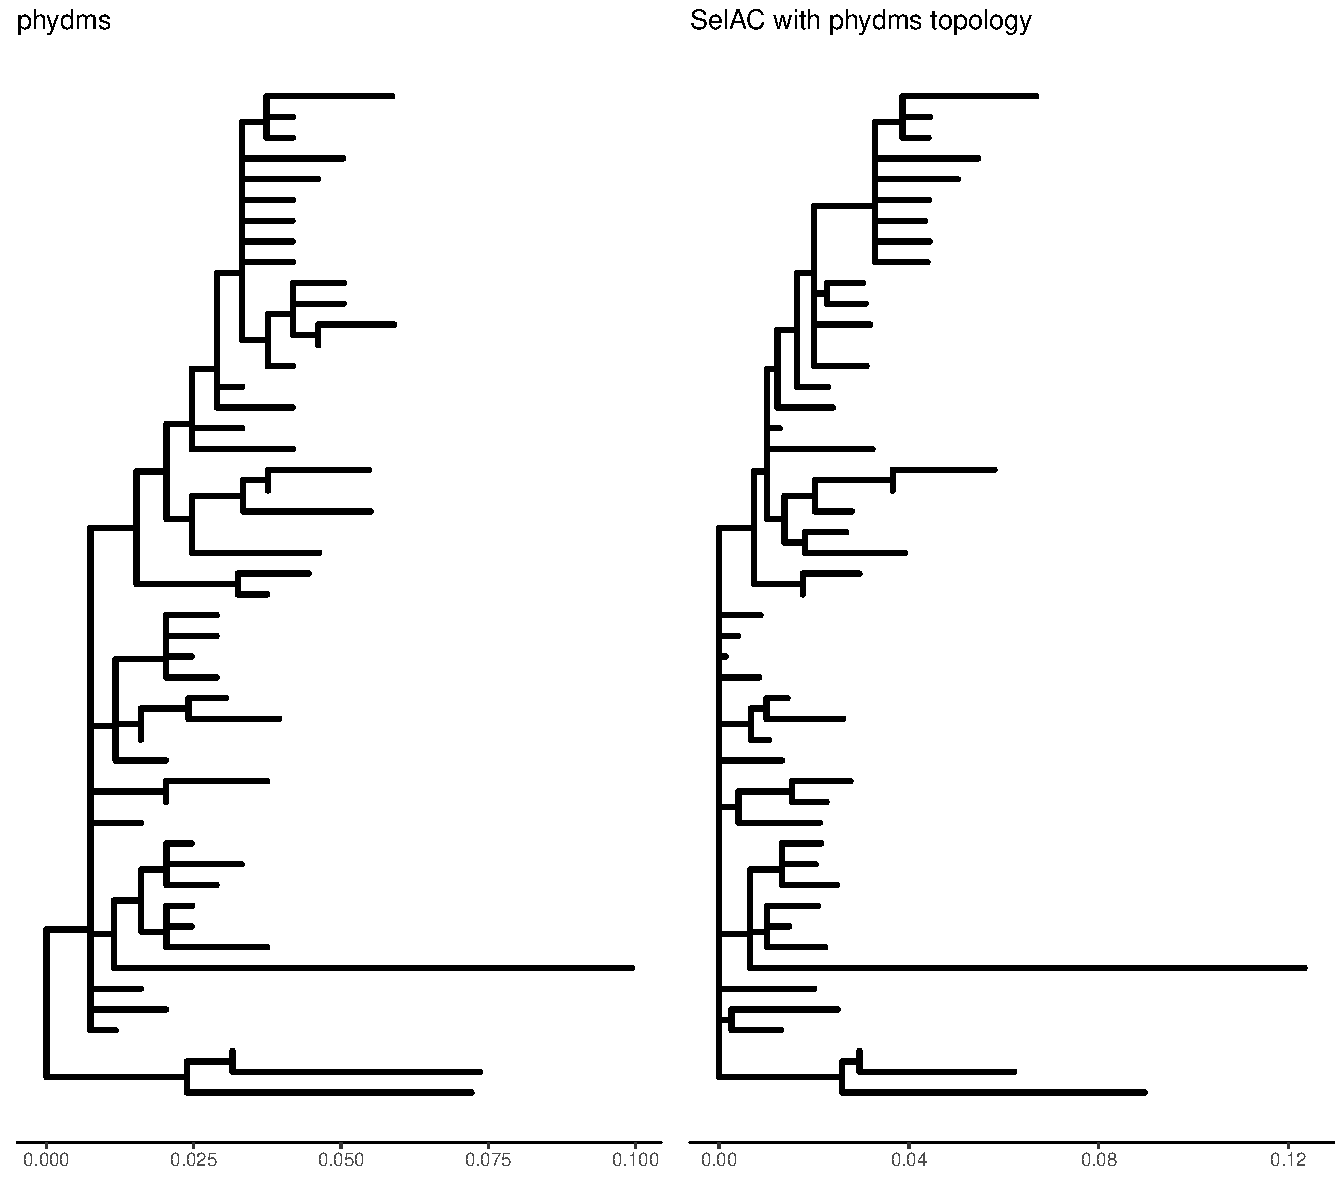
\includegraphics[width=\textwidth]{ch4/selac_top_comp.pdf}
	\caption{Phylogenies resulting from phydms, and \selac using the \phydms topology.}
	\label{fig:phylo_comp}
\end{figure}
\doublespacing
